
%\documentclass[11pts,a4paper,amsmath,amssymb,floatfix]{article}%{report}%{book}
\documentclass[12pts,a4paper,amsmath,amssymb,floatfix]{article}%{report}%{book}
\usepackage{graphicx,wrapfig,pdfpages}% Include figure files
%\usepackage{dcolumn,enumerate}% Align table columns on decimal point
\usepackage{enumerate,enumitem}% Align table columns on decimal point
\usepackage{bm,dpfloat}% bold math
\usepackage[pdftex,bookmarks,colorlinks=true,urlcolor=rltblue,citecolor=blue]{hyperref}
\usepackage{amsfonts,amsmath,amssymb,stmaryrd,indentfirst}
\usepackage{times,psfrag}
\usepackage{natbib}
\usepackage{color}
\usepackage{units}
\usepackage{rotating}
\usepackage{multirow}
\usepackage[version=3]{mhchem}


\usepackage{pifont}
\usepackage{subfigure}
\usepackage{subeqnarray}
\usepackage{ifthen}

\usepackage{supertabular}
\usepackage{moreverb}
\usepackage{listings}
\usepackage{palatino}
%\usepackage{doi}
\usepackage{longtable}
\usepackage{float}
\usepackage{perpage}
\MakeSorted{figure}
%\usepackage{pdflscape}


%\usepackage{booktabs}
%\newcommand{\ra}[1]{\renewcommand{\arraystretch}{#1}}


\definecolor{rltblue}{rgb}{0,0,0.75}


%\usepackage{natbib}
\usepackage{fancyhdr} %%%%
\pagestyle{fancy}%%%%
% with this we ensure that the chapter and section
% headings are in lowercase
%%%%\renewcommand{\chaptermark}[1]{\markboth{#1}{}}
\renewcommand{\sectionmark}[1]{\markright{\thesection\ #1}}
\fancyhf{} %delete the current section for header and footer
\fancyhead[LE,RO]{\bfseries\thepage}
\fancyhead[LO]{\bfseries\rightmark}
\fancyhead[RE]{\bfseries\leftmark}
\renewcommand{\headrulewidth}{0.5pt}
% make space for the rule
\fancypagestyle{plain}{%
\fancyhead{} %get rid of the headers on plain pages
\renewcommand{\headrulewidth}{0pt} % and the line
}

\def\newblock{\hskip .11em plus .33em minus .07em}
\usepackage{color}

%\usepackage{makeidx}
%\makeindex

\setlength\textwidth      {16.cm}
\setlength\textheight     {22.6cm}
\setlength\oddsidemargin  {-0.3cm}
\setlength\evensidemargin {0.3cm}

\setlength\headheight{14.49998pt} 
\setlength\topmargin{0.0cm}
\setlength\headsep{1.cm}
\setlength\footskip{1.cm}
\setlength\parskip{0pt}
\setlength\parindent{0pt}



\usepackage[T1]{fontenc}
\usepackage[utf8]{inputenc}
\usepackage{lmodern}
\usepackage[version=3]{mhchem}


\makeatletter
\newcounter{reaction}
%%% >> for article <<
\renewcommand\thereaction{C\,\arabic{reaction}}
%%% << for article <<
%%% >> for report and book >>
%\renewcommand\thereaction{C\,\thechapter.\arabic{reaction}}
%\@addtoreset{reaction}{chapter}
%%% << for report and book <<
\newcommand\reactiontag{\refstepcounter{reaction}\tag{\thereaction}}
\newcommand\reaction@[2][]{\begin{equation}\ce{#2}%
\ifx\@empty#1\@empty\else\label{#1}\fi%
\reactiontag\end{equation}}
\newcommand\reaction@nonumber[1]{\begin{equation*}\ce{#1}%
\end{equation*}}
\newcommand\reaction{\@ifstar{\reaction@nonumber}{\reaction@}}
\makeatother 




%%%
%%% Headers and Footers
\lhead[] {\text{\small{EG5597 -- Advanced Chemical Engineering}}} 
\rhead[] {{\text{\small{Tutorial 01 (2014/15)}}}}
%\chead[] {\text{\small{Session 2012/13}}} 
\lfoot[]{Dr Jeff Gomes}
%\cfoot[\thepage]{\thepage} 
\rfoot[\text{\small{\thepage}}]{\thepage}
\renewcommand{\headrulewidth}{0.8pt}


%%%
%%% space between lines
%%%
\renewcommand{\baselinestretch}{1.5}

\newenvironment{VarDescription}[1]%
  {\begin{list}{}{\renewcommand{\makelabel}[1]{\textbf{##1:}\hfil}%
    \settowidth{\labelwidth}{\textbf{#1:}}%
    \setlength{\leftmargin}{\labelwidth}\addtolength{\leftmargin}{\labelsep}}}%
  {\end{list}}

%%%%%%%%%%%%%%%%%%%%%%%%%%%%%%%%%%%%%%%%%%%
%%%%%%                              %%%%%%%
%%%%%%      NOTATION SECTION        %%%%%%%
%%%%%%                              %%%%%%%
%%%%%%%%%%%%%%%%%%%%%%%%%%%%%%%%%%%%%%%%%%%

% Text abbreviations.
\newcommand{\ie}{{\em{i.e., }}}
\newcommand{\eg}{{\em{e.g., }}}
\newcommand{\wrt}{with respect to}
\newcommand{\lhs}{left hand side}
\newcommand{\rhs}{right hand side}
% Commands definining mathematical notation.

% This is for quantities which are physically vectors.
\renewcommand{\vec}[1]{{\mbox{\boldmath$#1$}}}
% Physical rank 2 tensors
\newcommand{\tensor}[1]{\overline{\overline{#1}}}
% This is for vectors formed of the value of a quantity at each node.
\newcommand{\dvec}[1]{\underline{#1}}
% This is for matrices in the discrete system.
\newcommand{\mat}[1]{\mathrm{#1}}


\DeclareMathOperator{\sgn}{sgn}
\newtheorem{thm}{Theorem}[section]
\newtheorem{lemma}[thm]{Lemma}

%\newcommand\qed{\hfill\mbox{$\Box$}}
\newcommand{\re}{{\mathrm{I}\hspace{-0.2em}\mathrm{R}}}
\newcommand{\inner}[2]{\langle#1,#2\rangle}
\renewcommand\leq{\leqslant}
\renewcommand\geq{\geqslant}
\renewcommand\le{\leqslant}
\renewcommand\ge{\geqslant}
\renewcommand\epsilon{\varepsilon}
\newcommand\eps{\varepsilon}
\renewcommand\phi{\varphi}
\newcommand{\bmF}{\vec{F}}
\newcommand{\bmphi}{\vec{\phi}}
\newcommand{\bmn}{\vec{n}}
\newcommand{\bmns}{{\textrm{\scriptsize{\boldmath $n$}}}}
\newcommand{\bmi}{\vec{i}}
\newcommand{\bmj}{\vec{j}}
\newcommand{\bmk}{\vec{k}}
\newcommand{\bmx}{\vec{x}}
\newcommand{\bmu}{\vec{u}}
\newcommand{\bmv}{\vec{v}}
\newcommand{\bmr}{\vec{r}}
\newcommand{\bma}{\vec{a}}
\newcommand{\bmg}{\vec{g}}
\newcommand{\bmU}{\vec{U}}
\newcommand{\bmI}{\vec{I}}
\newcommand{\bmq}{\vec{q}}
\newcommand{\bmT}{\vec{T}}
\newcommand{\bmM}{\vec{M}}
\newcommand{\bmtau}{\vec{\tau}}
\newcommand{\bmOmega}{\vec{\Omega}}
\newcommand{\pp}{\partial}
\newcommand{\kaptens}{\tensor{\kappa}}
\newcommand{\tautens}{\tensor{\tau}}
\newcommand{\sigtens}{\tensor{\sigma}}
\newcommand{\etens}{\tensor{\dot\epsilon}}
\newcommand{\ktens}{\tensor{k}}
\newcommand{\half}{{\textstyle \frac{1}{2}}}
\newcommand{\tote}{E}
\newcommand{\inte}{e}
\newcommand{\strt}{\dot\epsilon}
\newcommand{\modu}{|\bmu|}
% Derivatives
\renewcommand{\d}{\mathrm{d}}
\newcommand{\D}{\mathrm{D}}
\newcommand{\ddx}[2][x]{\frac{\d#2}{\d#1}}
\newcommand{\ddxx}[2][x]{\frac{\d^2#2}{\d#1^2}}
\newcommand{\ddt}[2][t]{\frac{\d#2}{\d#1}}
\newcommand{\ddtt}[2][t]{\frac{\d^2#2}{\d#1^2}}
\newcommand{\ppx}[2][x]{\frac{\partial#2}{\partial#1}}
\newcommand{\ppxx}[2][x]{\frac{\partial^2#2}{\partial#1^2}}
\newcommand{\ppt}[2][t]{\frac{\partial#2}{\partial#1}}
\newcommand{\pptt}[2][t]{\frac{\partial^2#2}{\partial#1^2}}
\newcommand{\DDx}[2][x]{\frac{\D#2}{\D#1}}
\newcommand{\DDxx}[2][x]{\frac{\D^2#2}{\D#1^2}}
\newcommand{\DDt}[2][t]{\frac{\D#2}{\D#1}}
\newcommand{\DDtt}[2][t]{\frac{\D^2#2}{\D#1^2}}
% Norms
\newcommand{\Ltwo}{\ensuremath{L_2} }
% Basis functions
\newcommand{\Qone}{\ensuremath{Q_1} }
\newcommand{\Qtwo}{\ensuremath{Q_2} }
\newcommand{\Qthree}{\ensuremath{Q_3} }
\newcommand{\QN}{\ensuremath{Q_N} }
\newcommand{\Pzero}{\ensuremath{P_0} }
\newcommand{\Pone}{\ensuremath{P_1} }
\newcommand{\Ptwo}{\ensuremath{P_2} }
\newcommand{\Pthree}{\ensuremath{P_3} }
\newcommand{\PN}{\ensuremath{P_N} }
\newcommand{\Poo}{\ensuremath{P_1P_1} }
\newcommand{\PoDGPt}{\ensuremath{P_{-1}P_2} }

\newcommand{\metric}{\tensor{M}}
\newcommand{\configureflag}[1]{\texttt{#1}}

% Units
\newcommand{\m}[1][]{\unit[#1]{m}}
\newcommand{\km}[1][]{\unit[#1]{km}}
\newcommand{\s}[1][]{\unit[#1]{s}}
\newcommand{\invs}[1][]{\unit[#1]{s}\ensuremath{^{-1}}}
\newcommand{\ms}[1][]{\unit[#1]{m\ensuremath{\,}s\ensuremath{^{-1}}}}
\newcommand{\mss}[1][]{\unit[#1]{m\ensuremath{\,}s\ensuremath{^{-2}}}}
\newcommand{\K}[1][]{\unit[#1]{K}}
\newcommand{\PSU}[1][]{\unit[#1]{PSU}}
\newcommand{\Pa}[1][]{\unit[#1]{Pa}}
\newcommand{\kg}[1][]{\unit[#1]{kg}}
\newcommand{\rads}[1][]{\unit[#1]{rad\ensuremath{\,}s\ensuremath{^{-1}}}}
\newcommand{\kgmm}[1][]{\unit[#1]{kg\ensuremath{\,}m\ensuremath{^{-2}}}}
\newcommand{\kgmmm}[1][]{\unit[#1]{kg\ensuremath{\,}m\ensuremath{^{-3}}}}
\newcommand{\Nmm}[1][]{\unit[#1]{N\ensuremath{\,}m\ensuremath{^{-2}}}}

% Dimensionless numbers
\newcommand{\dimensionless}[1]{\mathrm{#1}}
\renewcommand{\Re}{\dimensionless{Re}}
\newcommand{\Ro}{\dimensionless{Ro}}
\newcommand{\Fr}{\dimensionless{Fr}}
\newcommand{\Bu}{\dimensionless{Bu}}
\newcommand{\Ri}{\dimensionless{Ri}}
\renewcommand{\Pr}{\dimensionless{Pr}}
\newcommand{\Pe}{\dimensionless{Pe}}
\newcommand{\Ek}{\dimensionless{Ek}}
\newcommand{\Gr}{\dimensionless{Gr}}
\newcommand{\Ra}{\dimensionless{Ra}}
\newcommand{\Sh}{\dimensionless{Sh}}
\newcommand{\Sc}{\dimensionless{Sc}}


% Journals
\newcommand{\IJHMT}{{\it International Journal of Heat and Mass Transfer}}
\newcommand{\NED}{{\it Nuclear Engineering and Design}}
\newcommand{\ICHMT}{{\it International Communications in Heat and Mass Transfer}}
\newcommand{\NET}{{\it Nuclear Engineering and Technology}}
\newcommand{\HT}{{\it Heat Transfer}}   
\newcommand{\IJHT}{{\it International Journal for Heat Transfer}}

\newcommand{\frc}{\displaystyle\frac}

\newlist{ExList}{enumerate}{1}
\setlist[ExList,1]{label={\bf Example 1.} {\bf \arabic*}}

\newlist{ProbList}{enumerate}{1}
\setlist[ProbList,1]{label={\bf Problem 1.} {\bf \arabic*}}

%%%%%%%%%%%%%%%%%%%%%%%%%%%%%%%%%%%%%%%%%%%
%%%%%%                              %%%%%%%
%%%%%% END OF THE NOTATION SECTION  %%%%%%%
%%%%%%                              %%%%%%%
%%%%%%%%%%%%%%%%%%%%%%%%%%%%%%%%%%%%%%%%%%%


% Cause numbering of subsubsections. 
%\setcounter{secnumdepth}{8}
%\setcounter{tocdepth}{8}

\setcounter{secnumdepth}{4}%
\setcounter{tocdepth}{4}%


\begin{document}



\begin{enumerate}[label=\bfseries Problem \arabic*]

%%%
%%%
%%%
\item\label{Tut01:FDM} An engineer consultant is hired to help in the design of a new F1-car front-wing air-foil. The back part of the air-foil is in contact with the car nose (chassis) and the outer part is in contact with flowing air. At first, the engineer needs to know the temperature profile across the wing as the temperature of chassis is at 200$^{o}$C and the ambient air temperature is at 20$^{o}$C. Heat loss in the tip of the air-foil is assumed negligible. The engineer also assumed that air is incompressible and that the nose and air temperatures are constant. The temperature across the air-foil can be expressed as an 1-D elliptic partial differential equation,
\begin{displaymath}
\frc{\partial^{2} T}{\partial x^{2}} -\alpha T = -\alpha T_{\text{amb}}
\end{displaymath} 
where $\alpha=20\;^{\text{o}}$C.m$^{-2}$ and $T_{\text{amb}}$ is the temperature of the flowing air. Estimate the temperature profile at 4 nodes equally spaced in the air-foil of length $L=0.30$m.

%%%
%%%
%%%
\item\label{Tut01:BCs} Define the 3 types of boundary conditions used to solve PDEs.


%%%
%%%
%%%
\item\label{Tut01:PDE_Taylor}A particular case of PDE's is
\begin{displaymath}
u_{t}+\alpha u_{x} = \kappa u_{xx}
\end{displaymath}
that represents advection-diffusion problems (with constant coefficients $\alpha$ and $\kappa$) with a number of applications in fluid and solid mechanics. Demonstrate that the advection term (in 1D and assuming regular grid) is
\begin{displaymath}
\frc{\partial u}{\partial x}=\frc{u_{i+1}-u_{i}}{\Delta x_{i}} + \mathcal{O}\left(\Delta x\right)
\end{displaymath}
using Taylor's expansion.


%%%
%%%
%%%
\item\label{Tut01:PDE_FDM} A team of process chemical engineers is tasked to design a stirred tank with optimal mixing performance to synthetise product-$\mathcal{X}$. The team initially needs to understand the flow dynamics of Newtonian and incompressible fluids in the tank by solving advection-diffusion transport equations with a commercial CFD. In order to validate the initial assumptions of the fluid and the problem, they decided to perform a hand-calculation in a 1D system. Chemical species are advected at velocity $u_{x}=0.50$ m/s with time-step size $\left(\Delta t\right)$ of $3$s through $60$ m. Discretising the transport equation in space and time the concentration can be calculated, using FDM, as
\begin{displaymath}
\mathcal{C}_{i}^{j+1}=\mathcal{C}_{i}^{j} - \frac{u\Delta t}{\Delta x }\left(\mathcal{C}_{i+1}^{j}-\mathcal{C}_{i}^{j}\right)
\end{displaymath}
where $i\in\left\{1,2,...,N_{x}\right\}$ and $j\in\left\{0,1,...,k\right\}$ are spatial- and time-increment indexes, respectively. The system is initially at rest. Assume:
\begin{itemize}
\item The domain is divided into $N_{x}=4$ nodes;
\item Initial condition is given by,
\[
\mathcal{C}\left(x,t=0\right)=
\left\{\begin{array}{l l}
0.1                               & \text{for } x < 20 \\
0.075 + e^{-0.01\left(x-45\right)^{2}} & \text{for } 20 \le x \le 40 \\
0.0 & \text{elsewhere.}
\end{array}\right.\]
\item The {\it ghost-node}: $x_{N_{x}+1}=x_{N_{x}}$
\end{itemize}
Calculate $\mathcal{C}_{i}^{1}$ (i.e., at $j = 1$ -- a-d).\\
%\begin{center}
\hbox{\hspace{4.cm}\begin{tabular}{||c | c c c c ||}
\hline\hline
{\bf i} & 1   & 2    & 3   &  4   \\
\hline\hline
$x_{1}$ &   &   &  &  \\
$\mathcal{C}_{i}^{0}$ &  & &  &  \\
$\mathcal{C}_{i}^{1}$ & (a) & (b) & (c) & (d) \\
\hline\hline
\end{tabular}}
%\end{center}

%%%
%%%
%%%
\item\label{Tut01:PDE_FDM_Formulation} The same engineering team decided that the most efficient way to synthetise product-$\mathcal{X}$ is to use a series of CSTRs (continuous stirred tank reactor). For the initial assessment prior to the CSTR design, they decided to investigate the flow dynamics in one CSTR assuming constant inlet and outlet mass flows (Fig.~\ref{fig1}). The system is assumed adiabatic (thus no heat transfer to the surroundings). In the reactor, a fluid $A$ (pure at liquid phase) reacts with a fluid $B$ (pure at gas phase) producing $\mathcal{X}$ with reaction rate of $\mathcal{R}$ until the system reach equilibrium with equilibrium constant of $K_{e}$,
  \reaction[chemreaction:reaction]{ A(l) +  B(g) <=>[\text{K$_{e}$}] \mathcal{X}(l)}
Fluid mixing is a key aspect in the design of a high-performace CSTR, therefore 4 baffles and a stirrer are included in the system. Before the reactor (and required associated facilities) design stage starts, the team needs to determine a few key-variables profiles (spatial and temporal): ${\bf u}\left(\underline{x},t\right)$, $P\left(\underline{x},t\right)$, $T\left(\underline{x},t\right)$ and $\mathcal{C}_{i}\left(\underline{x},t\right)$ (where $i\in\left\{1,2,\cdots\right\}$ corresponds to the different chemical species in solution). Describe the mathematical and physical formulations for the problem with all the necessary assumptions. This must include all steps from the initial formulation, and pre-processing to the begining of the simulation.
\begin{figure}[h]
  \begin{center}
    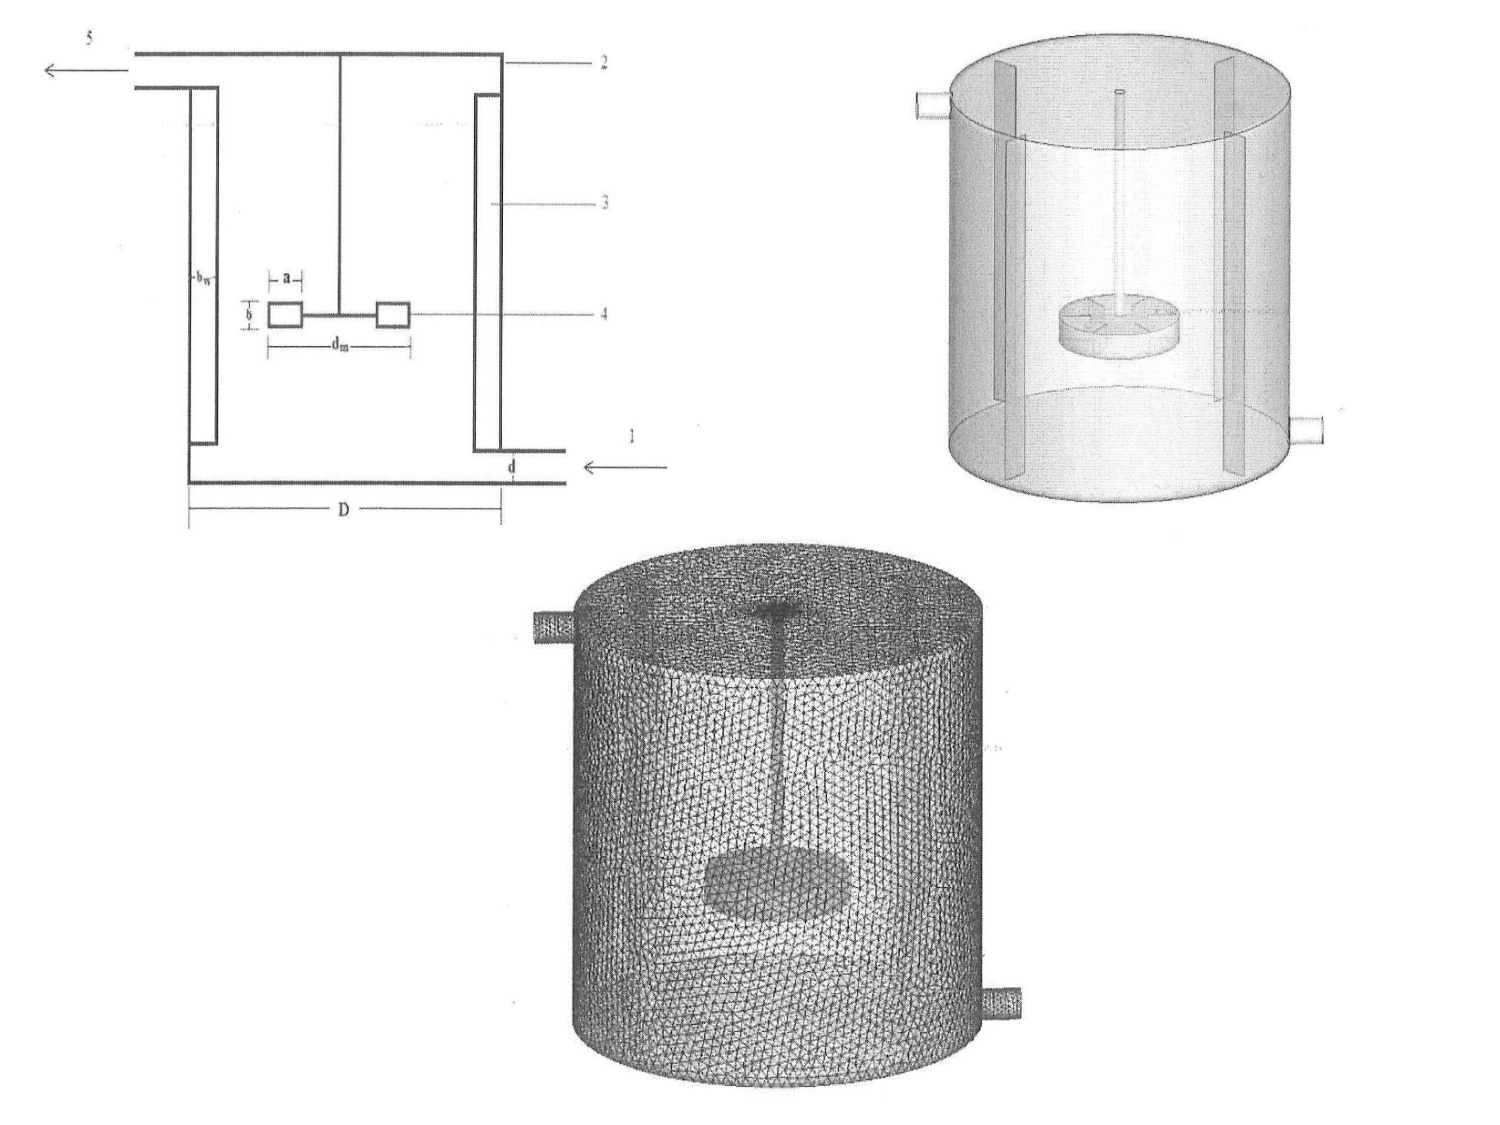
\includegraphics[clip,width=0.79\textwidth]{Figs/Tutorial_CSTR}
  \end{center}\caption{Schematics of the CSTR (\ref{Tut01:PDE_FDM_Formulation}.)\label{fig1}}
\end{figure}


\end{enumerate}



\clearpage

%{
%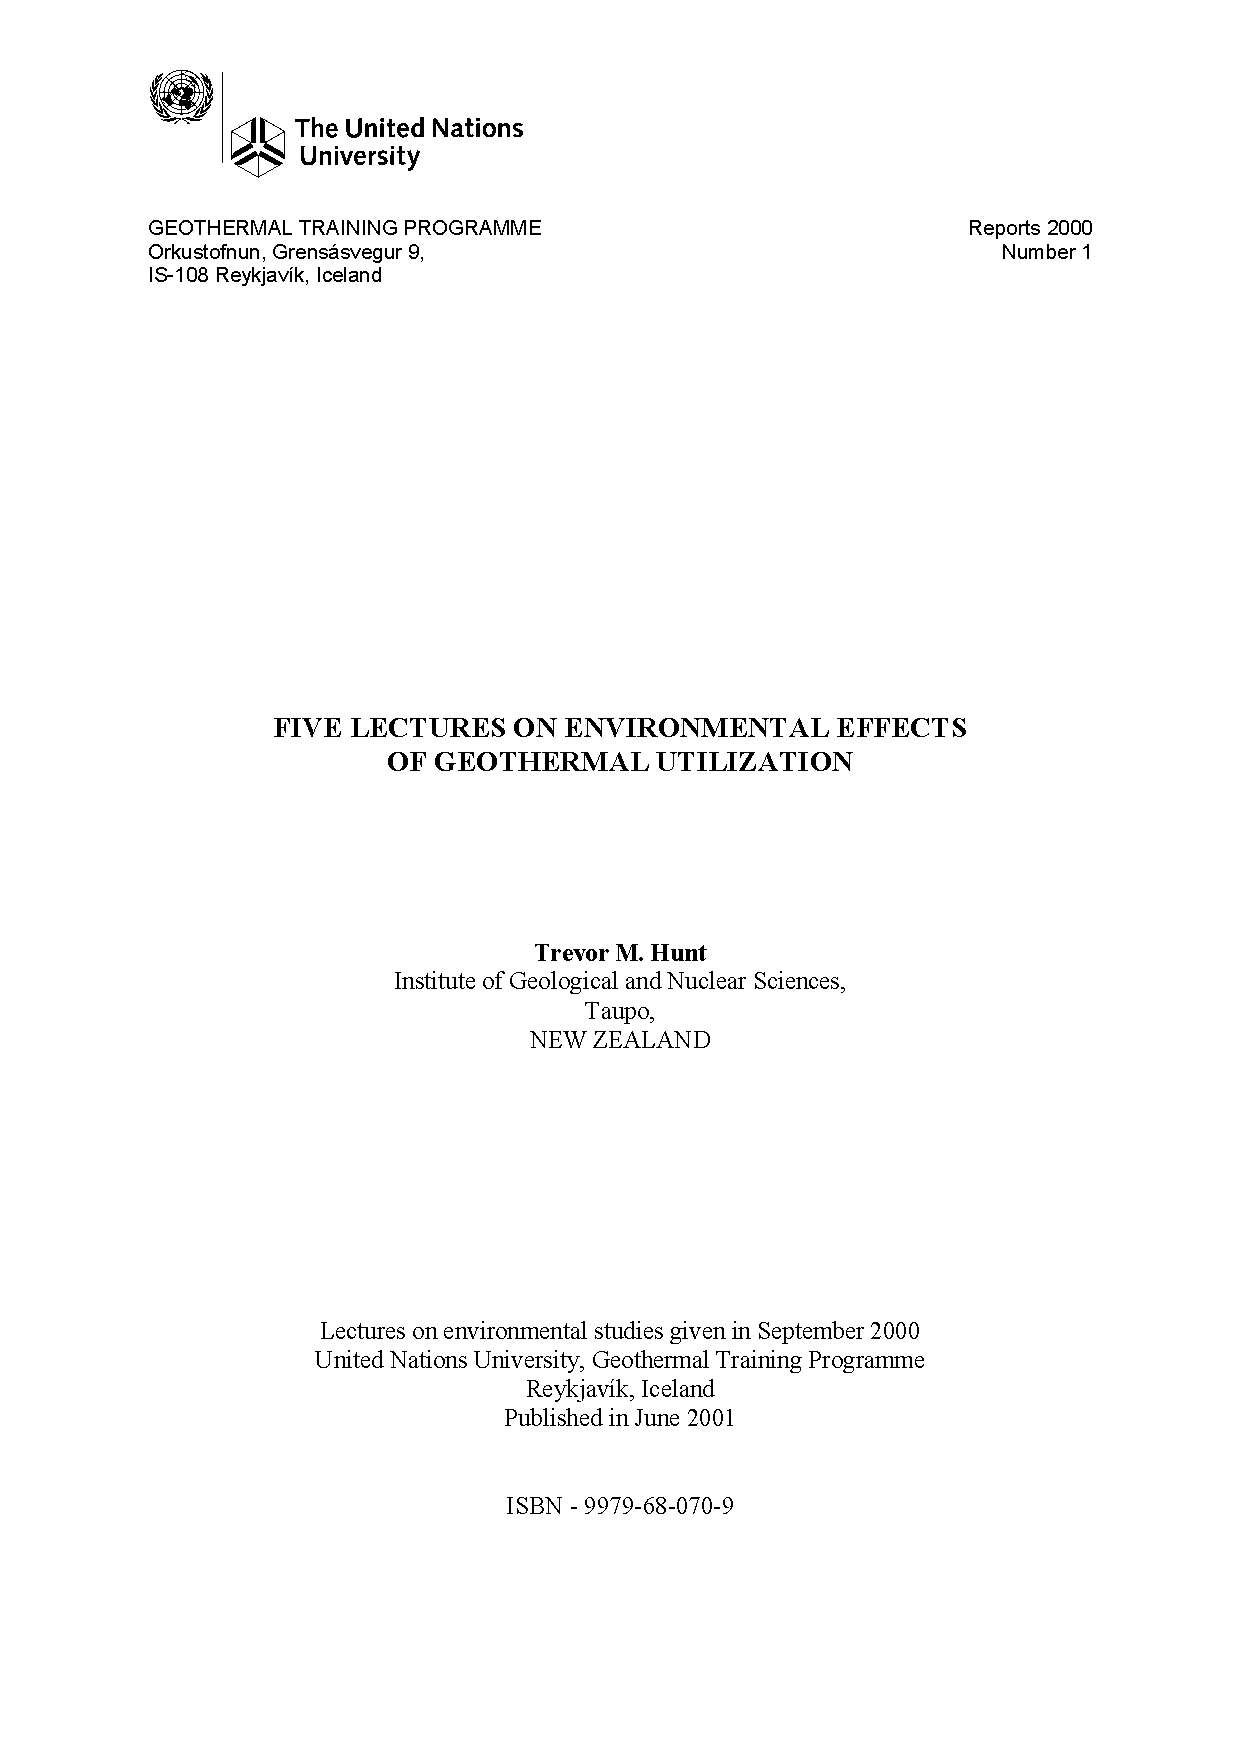
\includepdf[pages=-,fitpaper, angle=0]{./HuntSelect.pdf}
%}

\end{document}
